\begin{figure}[h]
\centering
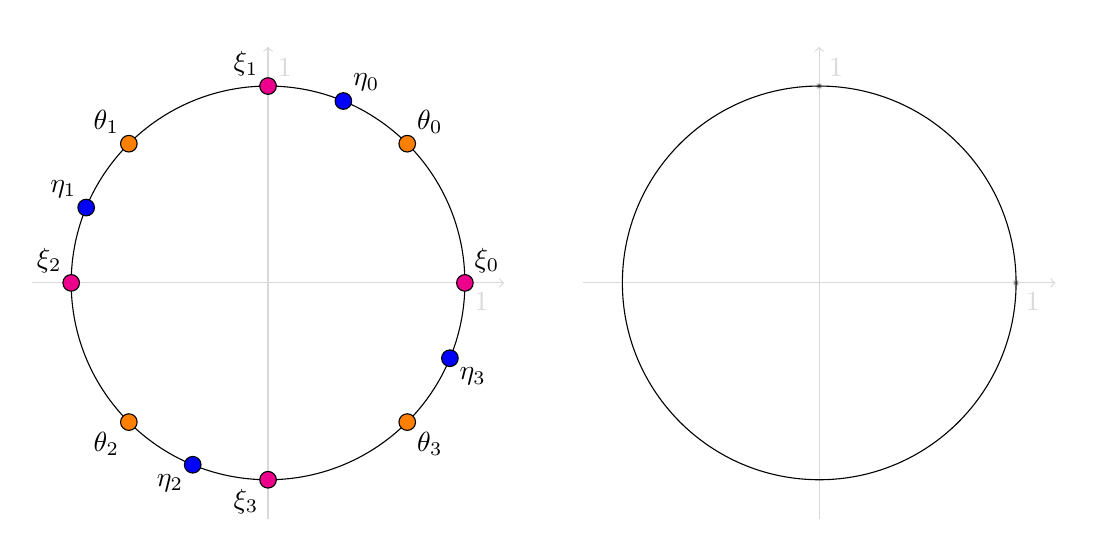
\begin{tikzpicture}
  % Gray coordinate system
  \draw[gray!30,->] (-3,0) -- (3,0) node[right] {$\re$};
  \draw[gray!30,->] (0,-3) -- (0,3) node[above] {$\im$};
  \draw[gray!30,->] (4,0) -- (10,0) node[right] {$\re$};
  \draw[gray!30,->] (7,-3) -- (7,3) node[above] {$\im$};
  \draw[gray!30,fill=gray] (2.5,0) circle (1pt) node[below right] {1};
  \draw[gray!30,fill=gray] (0,2.5) circle (1pt) node[above right] {1};
  \draw[gray!30,fill=gray] (7,2.5) circle (1pt) node[above right] {1};
  \draw[gray!30,fill=gray] (9.5,0) circle (1pt) node[below right] {1};
  
  % Circle with radius 3cm
  \draw (0,0) circle (2.5cm);

  \draw (7,0) circle (2.5cm);
  
  % First dot at angle pi/4
  \draw[fill=orange] (45:2.5cm) circle (3pt) node[above right] {$\theta_0$};
  \draw[fill=orange] (135:2.5cm) circle (3pt) node[above left] {$\theta_1$};
  \draw[fill=orange] (225:2.5cm) circle (3pt) node[below left] {$\theta_2$};
  \draw[fill=orange] (315:2.5cm) circle (3pt) node[below right] {$\theta_3$};
  \draw[fill=magenta] (90:2.5cm) circle (3pt) node[above left] {$\xi_1$};
  \draw[fill=magenta] (180:2.5cm) circle (3pt) node[above left] {$\xi_2$};
  \draw[fill=magenta] (270:2.5cm) circle (3pt) node[below left] {$\xi_3$};
  \draw[fill=magenta] (0:2.5cm) circle (3pt) node[above right] {$\xi_0$};
  \draw[fill=blue] (67.5:2.5cm) circle (3pt) node[above right] {$\eta_0$};
  \draw[fill=blue] (157.5:2.5cm) circle (3pt) node[above left] {$\eta_1$};
  \draw[fill=blue] (247.5:2.5cm) circle (3pt) node[below left] {$\eta_2$};
  \draw[fill=blue] (337.5:2.5cm) circle (3pt) node[below right] {$\eta_3$};

\end{tikzpicture}
    \caption{The Stokes directions $\St(0,1)$ in orange, $\St(0,c)$ in blue and $\St(1,c)$ in pink for $c = 1+i \in \C$.}
    \label{fig:enter-label}
\end{figure}